\section*{Задание}
\addcontentsline{toc}{section}{Задание}

Разработать многопотоковый вариант программы моделирования лифтовой системы (см.
задание 8 из лаб. работы 1). При этом модели БН, ЛП и ЛГ выполняются в рамках
отдельных потоков программы.

Задание 8 из лаб. работы №1:

Разработать программу, моделирующую в реальном времени работу лифтовой системы
десятиэтажного дома, состоящей из блока управления БУ, пассажирского ЛП и
грузового ЛГ лифтов. БУ отслеживает текущее состояние лифтов, принимает вызовы
пассажиров на этажах, диспетчеризует движение лифтов (выбирает "ближайший",
направляет к пассажирам, тормозит на промежуточных этажах и т.п.), индицирует
состояние лифтов. Лифты исполняют команды находящихся в них пассажиров и команды
БУ. Скорость ЛП в два раза выше скорости ЛГ. Работа каждого элемента системы
(БН, ЛП и ЛГ) моделируется отдельным процессом. Клавиши "1"..."0" используются
для имитации клавиш вызова лифта на этажах здания. Следующий ряд клавиш
"q"..."p" имитирует кнопки внутри ЛП, а ряд "a"...":" - внутри ЛГ. Для обработки
нажатий клавиш использовать неканонический режим. Визуализация перемещения
лифтов може выглядить, например, след. образом.

\texttt{ЛП - - - - 2 - - - - -}

\texttt{ЛГ - - - - - - - - 0 -}

Здесь цифры индицируют количество пассажиров в лифте.


\newpage

\section*{Описание структуры программы}
\addcontentsline{toc}{section}{Описание структуры программы}

В реализации данной программы было использовано 4 потока: один координирующий,
два обновляющих состояние лифтов и один поток отображения.

Потоки работают с общим состоянием в виде двух лифтов, поэтому для их
синхронизации использовались взаимоисключающие блокировки (mutex). Для всех 4
потоков используется 1 общий мьютекс, блокирующий остальные потоки при доступе к
общим данным.

\begin{figure}[H]
    \centering
    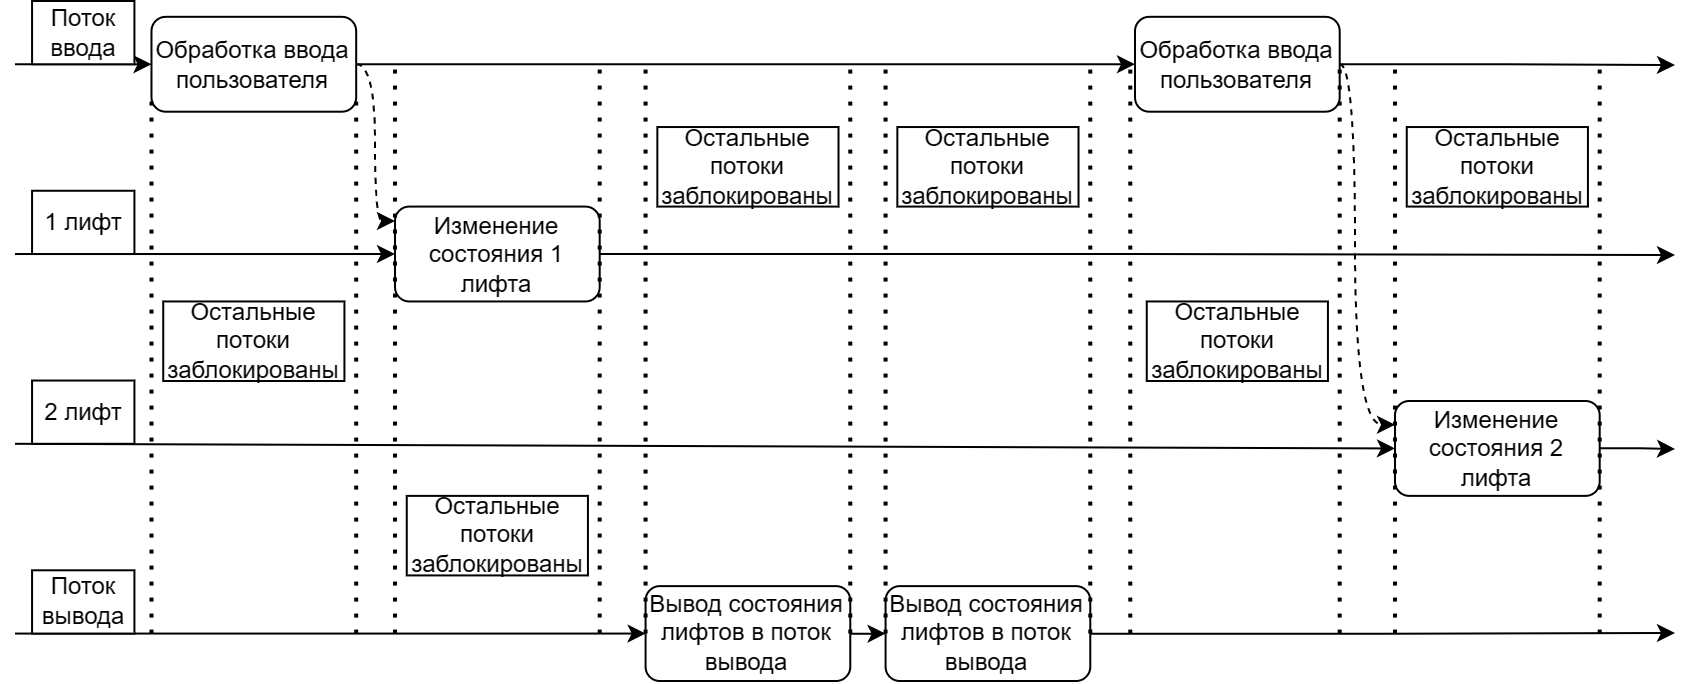
\includegraphics[width=\linewidth]{images/lab2_sync.drawio.png}
    \caption{Схема синхронизации потоков в программе}
    \label{fig:signals}
\end{figure}

Для работы с терминалом используется неканонический режим ввода с сокрытием
вводимых символов. Таким образом достигается большая <<интерактивность>> всего
процесса пользования.

\newpage

\section*{Блок-схема программы}
\addcontentsline{toc}{section}{Блок-схема программы}

\begin{figure}[H]
    \centering
    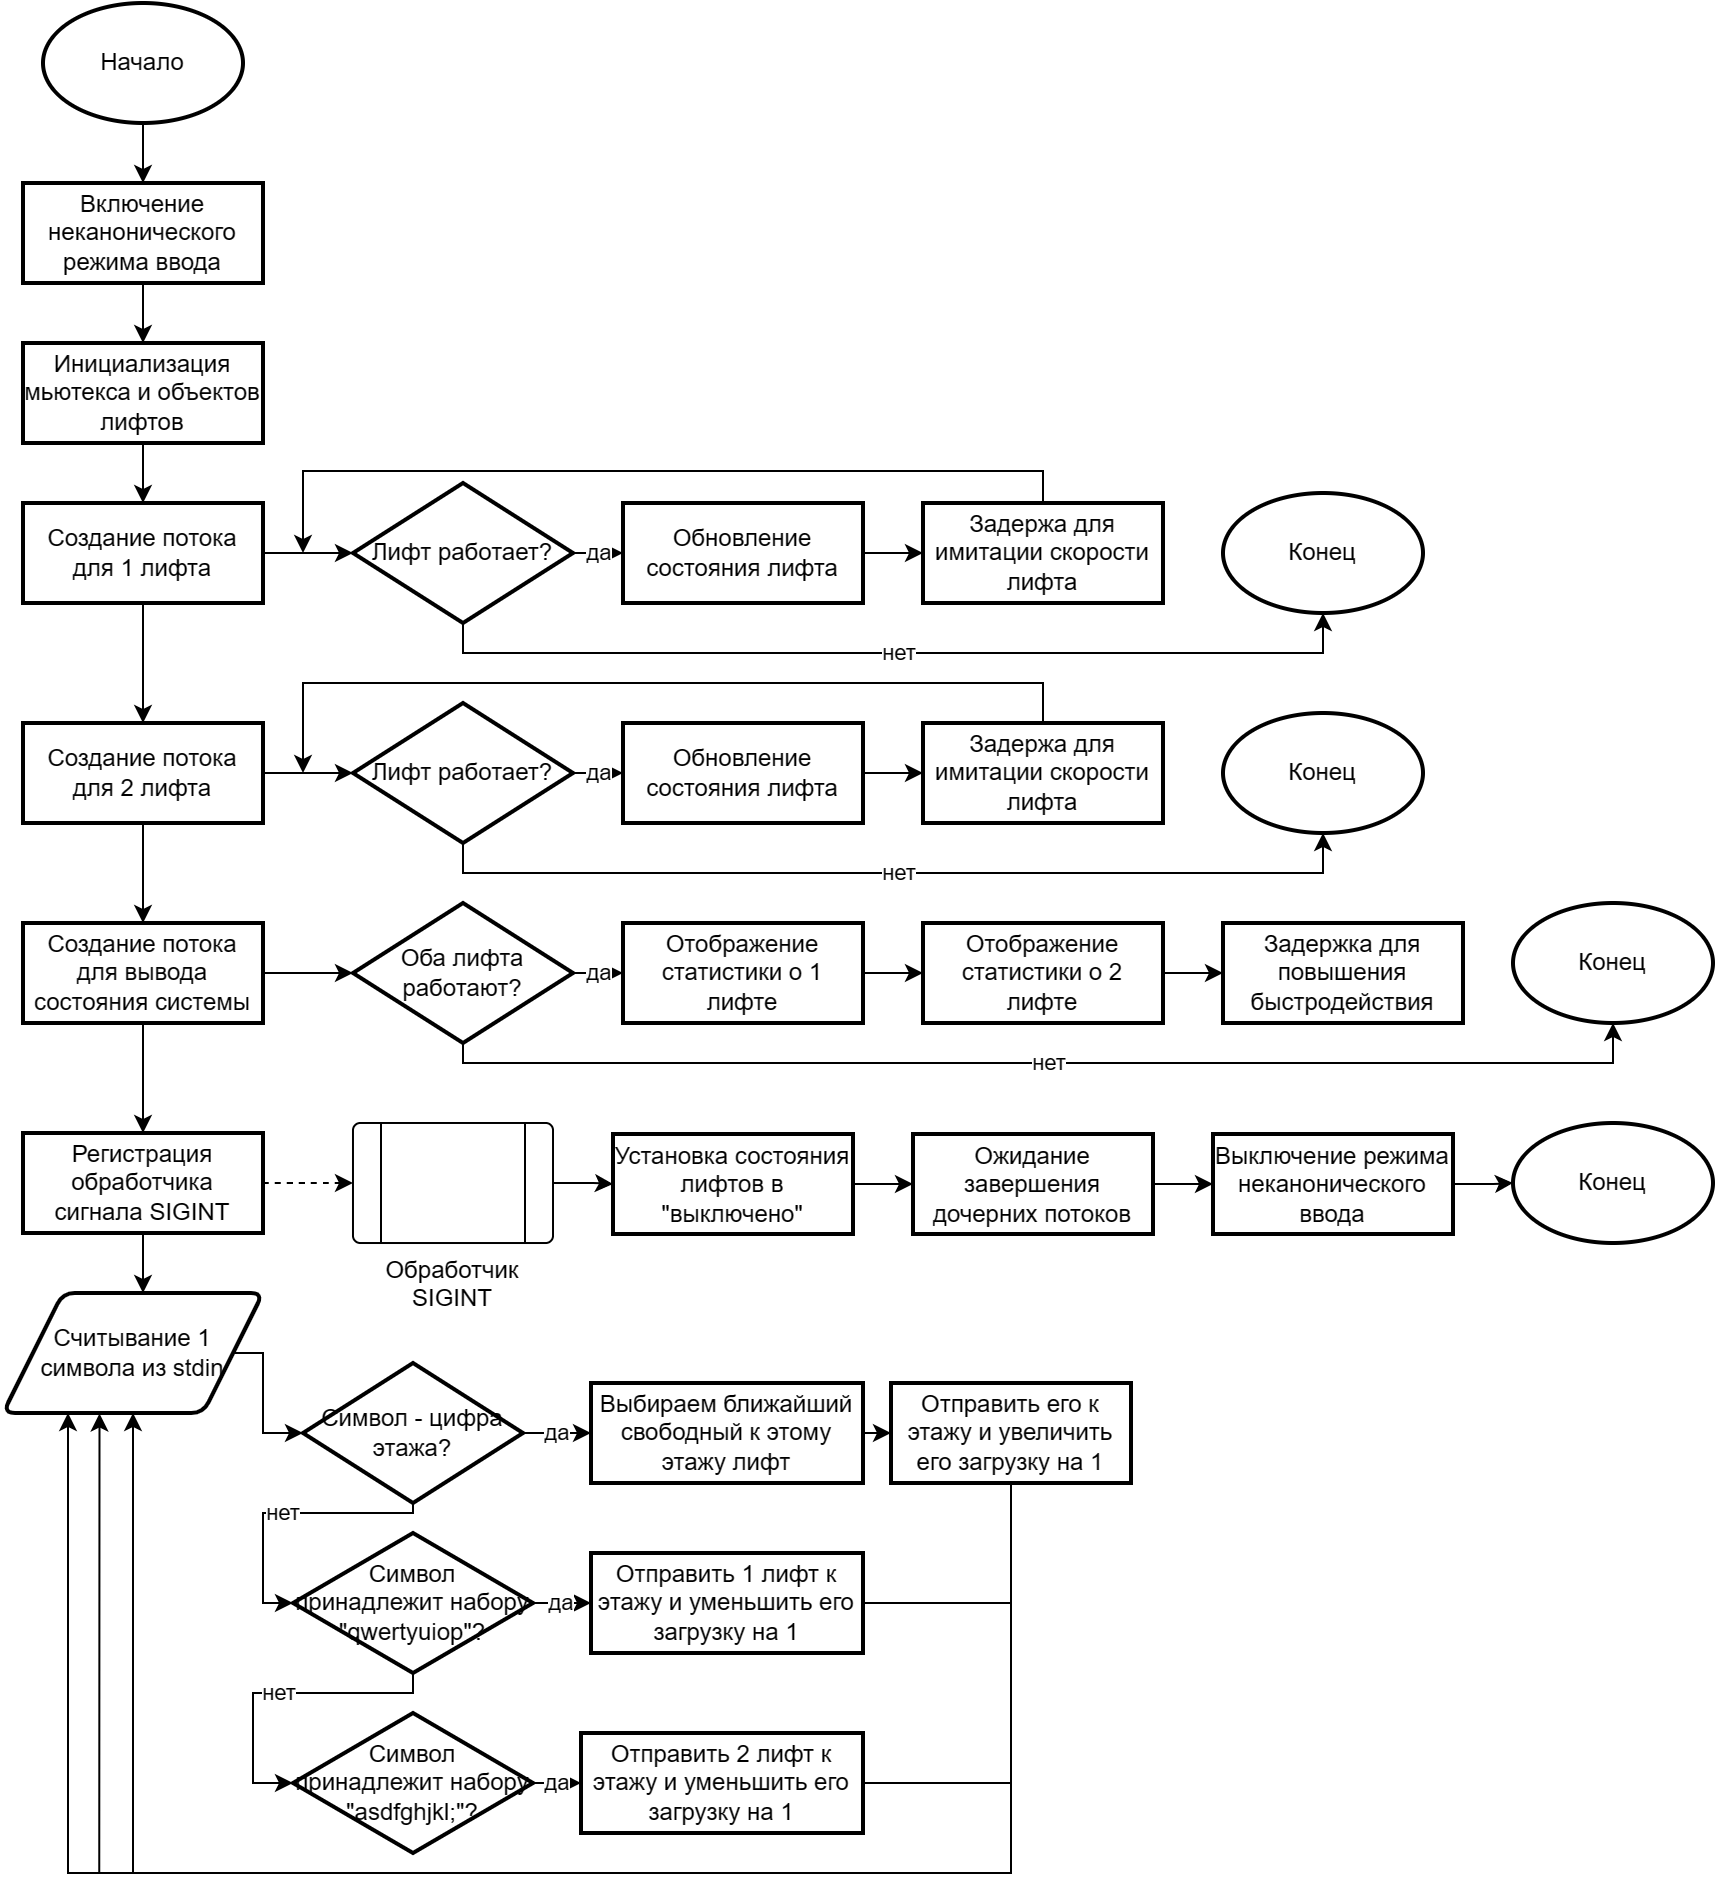
\includegraphics[width=0.75\linewidth]{images/lab2_block_scheme.drawio.png}
    \caption{Основная блок-схема программы}
    \label{fig:flowchart}
\end{figure}

\begin{figure}[H]
    \centering
    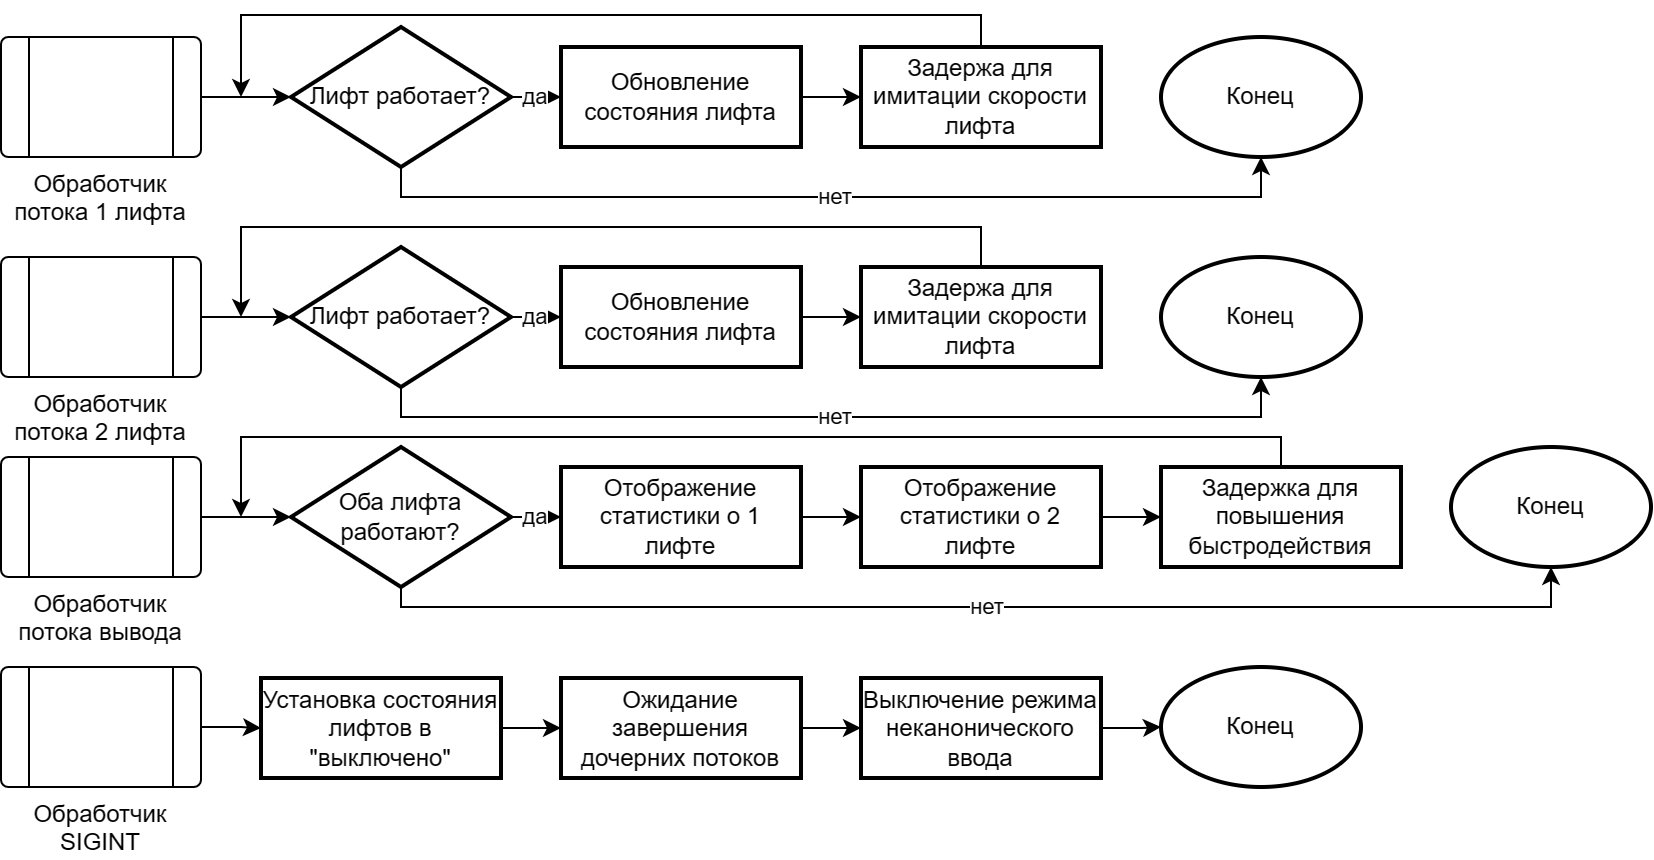
\includegraphics[width=0.9\linewidth]{images/lab2_handlers_scheme.drawio.png}
    \caption{Блок-схема обработчиков сигналов и потоков}
    \label{fig:handlers_flowchart}
\end{figure}

\newpage

\section*{Результат работы}
\addcontentsline{toc}{section}{Результат работы}

Так как программа меняет свой вывод в течении времени, то ниже приведены
несколько рисунков, отображающих различный вывод программы.

При вводе цифры, например, "5":

\begin{figure}[H]
    \centering
    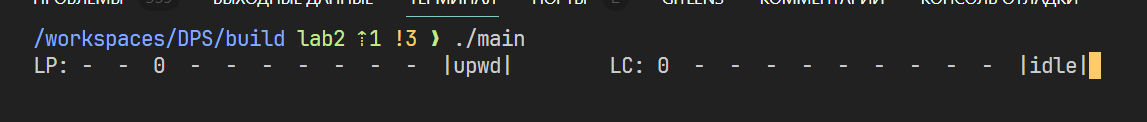
\includegraphics[width=0.8\linewidth]{images/lab2_output1.png}
    \caption{Вывод программы при перемещении одного из лифтов}
    \label{fig:output1}
\end{figure}

Когда лифт достиг нужного этажа:

\begin{figure}[H]
    \centering
    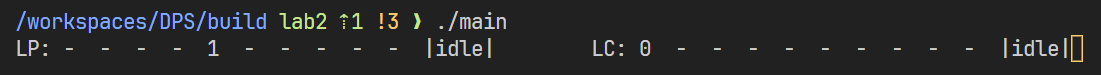
\includegraphics[width=0.8\linewidth]{images/lab2_output2.png}
    \caption{Вывод программы, при ожидающих лифтах}
    \label{fig:output2}
\end{figure}

Лифт можно отправить на другой этаж, чтобы тот разгрузился, для этого можно
нажать клавишу "u":

\begin{figure}[H]
    \centering
    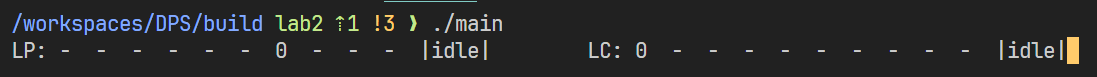
\includegraphics[width=0.8\linewidth]{images/lab2_output3.png}
    \caption{Вывод программы после разгрузки лифта}
    \label{fig:output3}
\end{figure}

\newpage

\appendix

\section*{Приложение}
\section*{Текст программы}
\addcontentsline{toc}{section}{Текст программы}

\begin{verbatim}
include/compare.h:

#pragma once

/// Used in comparing functions
typedef enum {
    Less = -1,
    Equal = 0,
    Greater = 1
} Ordering;

include/handler.h:

#pragma once

#include "lift.h"

/// Receives a passenger lift as a parameter [p] and updates it in infinite loop
/// Returns [NULL]
void *update_pass_lift(void *p);

/// Receives a cargo lift as a parameter [p] and updates it in infinite loop
/// Returns [NULL]
void *update_cargo_lift(void *p);

/// Receives an array of lifts of size 2 and displays it in infinite loop
/// Returns [NULL]
void *display_lifts(void *p);

/// Saves pointer to [mutex] for internal purposes
void init_handlers_system(pthread_mutex_t *mutex);

include/lift.h:

#pragma once

#include <pthread.h>
#include <stdbool.h>
#include <stdlib.h>

#include "compare.h"

#define MAX_FLOOR 10

typedef unsigned int Floor;

/// Idle - lift waits for commands - default state
/// Disabled - lift does not handle any commands
/// Upward - lift goes up
/// Downward - lift goes down
typedef enum { Downward, Upward, Idle, Disabled } LiftState;

typedef struct {
    Floor current_floor;
    Floor target_floor;
    /// Change of load when lift becomes idle again
    int load_change;
    unsigned int load;
    LiftState state;
} Lift;

/// Fills fields of [l] with default values
void init_lift(Lift *l);

/// Compares distances between two lifts against the [floor] and returns [Ordering]
Ordering compare(Lift a, Lift b, Floor floor);

/// Changes direction of the lift [l] when it's idle with respect to [floor]
void call_lift(Lift *l, Floor floor);

/// Checks if lift [l] is enabled and is not in idle state
bool is_busy(Lift l);

/// Returns nearest lift to [floor] from [lifts] using [compare] function, filtering all busy lifts
/// If all lifts are busy returns [NULL]
Lift *get_nearest_free(Lift *lifts, size_t size, Floor floor);

include/utils.h:

#pragma once

#include <stdio.h>
#include <stdlib.h>

#if DEBUG
#define DEBUG_PRINT(file, format, ...) fprintf(file, format, __VA_ARGS__)
#else
#define DEBUG_PRINT(...) 0
#endif

/// Checks if pointer is not null, otherwise returns [default] value and prints debug message to stderr (in debug mode
/// only)
#define RETURN_DEFAULT_IF_NULL(ptr, default)                                                                           \
    if ((ptr) == NULL) {                                                                                               \
        DEBUG_PRINT(stderr, "DEBUG: %s was NULL at %s:%d\n", #ptr, __FILE__, __LINE__);                                \
        return (default);                                                                                              \
    }                                                                                                                  \
    0

/// Checks if expr is non-negative integer, otherwise returns [on_error] code and prints debug message to stderr (in
/// debug mode only)
#define TRY_OR_ELSE(expr, on_error)                                                                                    \
    {                                                                                                                  \
        int code = expr;                                                                                               \
        if ((code) < 0) {                                                                                              \
            DEBUG_PRINT(stderr, "DEBUG: %s was lead to error %d at %s:%d", #expr, code, __FILE__, __LINE__);           \
            return on_error;                                                                                           \
        }                                                                                                              \
    }                                                                                                                  \
    0

/// Checks if expr is non-negative integer, otherwise forwards its error return code and prints debug message to stderr
/// (in debug mode only)
#define TRY_FORWARD(expr)                                                                                              \
    {                                                                                                                  \
        int code = expr;                                                                                               \
        if ((code) < 0) {                                                                                              \
            DEBUG_PRINT(stderr, "DEBUG: %s was lead to error %d at %s:%d", #expr, code, __FILE__, __LINE__);           \
            return code;                                                                                               \
        }                                                                                                              \
    }                                                                                                                  \
    0

/// Used in macro overloading
#define __TRY_OVERLOAD(_1, _2, name, ...) name

/// Checks if expr is non-negative integer, otherwise does action based on overload
/// SEE ALSO: [TRY_OR_ELSE], [TRY_FORWARD]
#define TRY(...) __TRY_OVERLOAD(__VA_ARGS__, TRY_OR_ELSE, TRY_FORWARD)(__VA_ARGS__)

/// Shortcut for write(..., <string literal>, sizeof(<same string literal>))
#define WRITE(fmt, message) write((fmt), (message), sizeof(message))

/// Shortcut for sizeof(<array type>) / sizeof(<type of item of array type>)
#define ARRAY_LEN(array) (sizeof(array) / sizeof(*(array)))

src/handler.c:

#include "handler.h"

#include <pthread.h>
#include <stdio.h>
#include <stdlib.h>
#include <unistd.h>

static const __useconds_t BASE_DELAY = 500 * 1000;

static pthread_mutex_t *mutex;

void init_handlers_system(pthread_mutex_t *mutex_) {
    mutex = mutex_;
}

/// Moves lift upwards or downwards or applies load change in idle state
static void do_update(Lift *lift) {
    pthread_mutex_lock(mutex);

    if (lift->current_floor == lift->target_floor) {
        lift->state = Idle;
        lift->load += lift->load_change;
        lift->load_change = 0;
    }
    call_lift(lift, lift->target_floor);

    if (lift->state == Downward)
        lift->current_floor--;
    if (lift->state == Upward)
        lift->current_floor++;

    pthread_mutex_unlock(mutex);
}

/// Displays current lift position to [stdout] with [prefix]
static void show(const Lift *l, const char *prefix) {
    pthread_mutex_lock(mutex);

    printf("%s:", prefix);

    for (Floor i = 1; i <= MAX_FLOOR; i++) {
        if (l->current_floor == i)
            printf(" %u ", l->load);
        else
            printf(" - ");
    }

    pthread_mutex_unlock(mutex);
}

void *update_pass_lift(void *p) {
    Lift *lift = p;
    while (lift->state != Disabled) {
        do_update(lift);

        usleep(BASE_DELAY);
    }

    return NULL;
}

void *update_cargo_lift(void *p) {
    Lift *lift = p;
    while (lift->state != Disabled) {
        do_update(lift);

        usleep(2 * BASE_DELAY);
    }

    return NULL;
}

/// Returns string representation of lift's state
static const char *display_state(LiftState state) {
    if (state == Disabled)
        return "dsbd";
    else if (state == Idle)
        return "idle";
    else if (state == Downward)
        return "down";

    return "upwd";
}

void *display_lifts(void *p) {
    Lift *lifts = p;

    while (lifts[0].state != Disabled || lifts[1].state != Disabled) {
        printf("\r");

        show(&lifts[0], "LP");
        printf(" |%s|\t", display_state(lifts[0].state));
        show(&lifts[1], "LC");
        printf(" |%s|", display_state(lifts[1].state));

        fflush(stdout);

        usleep(BASE_DELAY / 2);
    }

    return NULL;
}

src/lift.c:

#include "lift.h"

/// Gets a distance between current floor of lift and specified floor [b] with respect of lift's state
static unsigned int dist(Lift a, Floor b) {
    switch (a.state) {
    case Idle:
        if (a.current_floor > b)
            return a.current_floor - b;
        return b - a.current_floor;
    case Downward:
        if (a.current_floor < b)
            return a.current_floor + b;
        return a.current_floor - b;
    case Upward:
        if (a.current_floor > b)
            return 2 * MAX_FLOOR - a.current_floor - b - 1;
        return b - a.current_floor;
    case Disabled:
        return -1;
    }
}

/// Compares two unsigned int values and returns [Ordering]
static Ordering compare_uint(unsigned int a, unsigned int b) {
    if (a < b)
        return Less;
    if (a == b)
        return Equal;
    return Greater;
}

Ordering compare(Lift a, Lift b, Floor floor) { return compare_uint(dist(a, floor), dist(b, floor)); }

void call_lift(Lift *l, Floor floor) {
    if (l->state == Idle) {
        if (l->current_floor > floor)
            l->state = Downward;
        else if (l->current_floor < floor)
            l->state = Upward;
    }
}

bool is_busy(Lift l) { return l.state != Idle && l.state != Disabled; }

void init_lift(Lift *l) {
    l->current_floor = 1;
    l->load = 0;
    l->state = Idle;
    l->target_floor = 1;
    l->load_change = 0;
}

Lift *get_nearest_free(Lift *lifts, size_t size, Floor floor) {
    if (size == 0)
        return NULL;

    Lift *current = lifts;
    for (size_t i = 1; i < size; i++) {
        if (is_busy(lifts[i]))
            continue;

        Ordering cmp = compare(*current, lifts[i], floor);

        if (cmp == Greater || is_busy(*current))
            current = &lifts[i];
    }

    return is_busy(*current) ? NULL : current;
}

src/main.c:

#include <pthread.h>
#include <signal.h>
#include <termios.h>
#include <unistd.h>

#include "handler.h"
#include "lift.h"
#include "utils.h"

/// Used in function exit code
typedef enum {
    ThreadCreateFailed = -1,
    TerminalProps = -2,
    MutexCreateFailed = -3,
    WrongStdin = -4,

    Ok = 0,
} Error;

typedef void *(*Handler)(void *);

struct termios save;
pthread_t threads[3];
Lift lifts[2];

/// Disables lifts and joins threads while they're exiting
/// Also reenables canon input
void graceful_shutdown(int _sig) {
    lifts[0].state = lifts[1].state = Disabled;

    pthread_join(threads[0], NULL);
    pthread_join(threads[1], NULL);
    pthread_join(threads[2], NULL);

    tcsetattr(STDIN_FILENO, TCSAFLUSH, &save);
    printf("\n");

    exit(0);
}

/// Checks if current session is in terminal, saves it state and sets non-canon type of input
/// ERRORS: [WrongStdin] if current session is not in terminal
///         [TerminalProps] if failed to save or to set terminal properties
Error disable_canon_input(struct termios *save) {
    if (!isatty(STDIN_FILENO)) {
        perror("stdin isn't a terminal");
        return WrongStdin;
    }

    struct termios tty;

    TRY(tcgetattr(STDIN_FILENO, save), TerminalProps);
    tty = *save;
    tty.c_lflag &= ~(ICANON | ECHO);
    tty.c_cc[VMIN] = 1;
    TRY(tcsetattr(STDIN_FILENO, TCSAFLUSH, &tty), TerminalProps);

    return Ok;
}

/// Runs a new thread with default attributes calling [handler] with [arg]
/// ERRORS: [ThreadCreateFailed] - if failed to create a thread with default attrs
Error open_thread(pthread_t *thread, Handler handler, void *arg) {
    pthread_attr_t attr;
    TRY(pthread_attr_init(&attr), ThreadCreateFailed);
    TRY(pthread_create(thread, &attr, handler, arg), ThreadCreateFailed);

    return Ok;
}

/// Initialises [mutex] with default attributes
/// ERRORS: [MutexCreateFailed] - if failed to create a mutex with default attrs
Error get_fresh_mutex(pthread_mutex_t *mutex) {
    pthread_mutexattr_t attr;
    TRY(pthread_mutexattr_init(&attr));
    TRY(pthread_mutex_init(mutex, &attr));

    return Ok;
}

/// Searches for [ch] in array of chars [alphabet] with size [size]
/// Returns index of the first char of [alphabet] when it's equals to [ch], otherwise returns -1
size_t find_index(const char alphabet[], size_t size, char ch) {
    for (size_t i = 0; i < size; i++)
        if (alphabet[i] == ch)
            return i;
    return -1;
}

/// Reacts on user's input by moving lifts to certain floors
/// In particular, if input in 0..9, moves the nearest lift to this floor
/// if input in [lp_control], moves the first lift
/// if input in [lc_control], moves the second lift
void manage_lifts(unsigned char c, pthread_mutex_t *busy_mutex) {
    static const char floor_control[] = "1234567890";
    static const char lp_control[] = "qwertyuiop";
    static const char lc_control[] = "asdfghjkl;";
    size_t index;

    if ((index = find_index(floor_control, sizeof(floor_control), c)) != -1) {
        Lift *nearest = get_nearest_free(lifts, 2, index + 1);
        if (!nearest)
            return;

        nearest->target_floor = index + 1;
        nearest->load_change = 1;
    } else if ((index = find_index(lp_control, sizeof(lp_control), c)) != -1 && lifts[0].load > 0) {
        lifts[0].target_floor = index + 1;
        lifts[0].load_change = -1;
    } else if ((index = find_index(lc_control, sizeof(lc_control), c)) != -1 && lifts[1].load > 0) {
        lifts[1].target_floor = index + 1;
        lifts[1].load_change = -1;
    }

    return;
}

/// Program's entry point. Initializes lifts, mutex and displaying system, opens 3 threads for handling user input and
/// reads user input in infinite loop
int main() {
    TRY(disable_canon_input(&save));

    pthread_mutex_t busy_mutex;
    TRY(get_fresh_mutex(&busy_mutex));

    init_lift(&lifts[0]);
    init_lift(&lifts[1]);
    init_handlers_system(&busy_mutex);

    TRY(open_thread(&threads[0], update_pass_lift, &lifts[0]));
    TRY(open_thread(&threads[1], update_cargo_lift, &lifts[1]));
    TRY(open_thread(&threads[2], display_lifts, lifts));

    signal(SIGINT, graceful_shutdown);

    while (true) {
        unsigned char next;
        read(STDIN_FILENO, &next, 1);
        size_t index;

        pthread_mutex_lock(&busy_mutex);

        manage_lifts(next, &busy_mutex);

        pthread_mutex_unlock(&busy_mutex);
    }
}

\end{verbatim}
